\documentclass[../main.tex]{subfiles}

\newcolumntype{C}[1]{>{\centering\arraybackslash}m{#1}}

\begin{document}
\chapter{Rezultaty}

Wszystkie metody przedstawione w poprzednich rozdziałach zostały zaimplementowane dla jednolitych, białych źródeł światła o prostokątnym kształcie. Rezultaty dla materiałów o stałym parametrze chropowatości na całej powierzchni, w danej grupie, zostały przedstawione w tabelach \ref{tab:results:metal} i \ref{tab:results:isolator}. Metoda referencyjna Monte-Carlo generuje $12 800$ próbek na piksel, w celu wyznaczenia wartości całki ($100$ iteracji po $128$ próbek na piksel każda). Obrazy wynikowe wygenerowane z pomocą tekstur opisujących niejednorodne materiały zróżnicowane pod względem normalnej, albedo, chropowatości czy też metaliczności znajdują się w tabeli \ref{tab:results:textured}. Tekstury te, są standardowymi zestawami obrazów przystosowanych do silników wspierających renderowanie bazowane na zjawiskach fizycznych.

Średnie czasy generowania jednej ramki obrazu w rozdzielczości $1024$x$1024$ pikseli znajdują się w tabeli \ref{tab:performance}. Platforma testowa składa się z procesora i5-8600K 3.60GHz, 16GB pamięci RAM i karty graficznej Nvidia GeForce GTX1080.

Na podstawie rezultatów możemy wyciągnąć wniosek, że metoda liniowo transformowanych konsinusów radzi sobie znacznie lepiej od metody chmury świateł punktowych, która nie daje dobrych rezultatów w pełnym spektrum chropowatości. Dla odpowiednio niskiego parametru wyraźnie widać strukturę światła powierzchniowego (rys. \ref{fig:results:pointManyLowAlpha}), a tego właśnie chcieliśmy uniknąć na samym początku. Zwiększanie ilości świateł poprawia wynik, ale bardzo wpływa na wydajność, jak wyraźnie widać w tabeli \ref{tab:performance}. Metoda liniowo transformowanych kosinusów nieznacznie różni się od metody referencyjnej i na pierwszy rzut oka wygląda bardzo podobnie, przez co utrata jakości percepcyjnie jest minimalna.

Wyznaczenie parametrów dla metody liniowo transformowanych kosinusów w obecnej implementacji zajmuje bardzo dużo czasu. Wygenerowanie mapy poglądowej o rozmiarze $64$x$64$ zajmuje około 9 godzin na platformie testowej. Podzbiór rezultatu nadający się do wizualnego porównania został umieszczony na rysunku \ref{fig:results:fitMatrix}, obrazek podglądowy dla każdego poszczególnego przybliżenia został dołączony do pracy wraz z kodem źródłowym.

\begin{figure}
    \centering
    \begin{subfigure}{0.45\textwidth}
        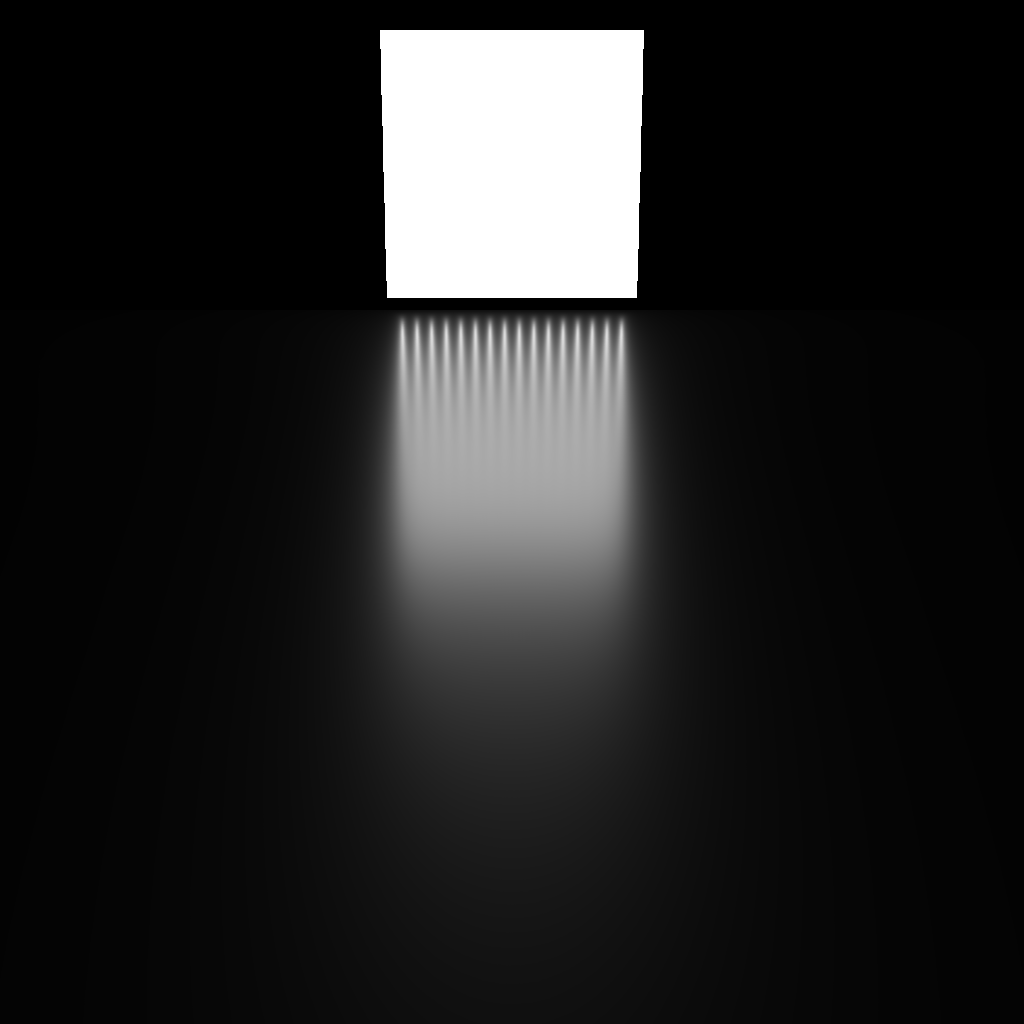
\includegraphics[width=\textwidth]{results/misc/point16x16-low-rough}
        \caption{16x16}
    \end{subfigure}
    \begin{subfigure}{0.45\textwidth}
        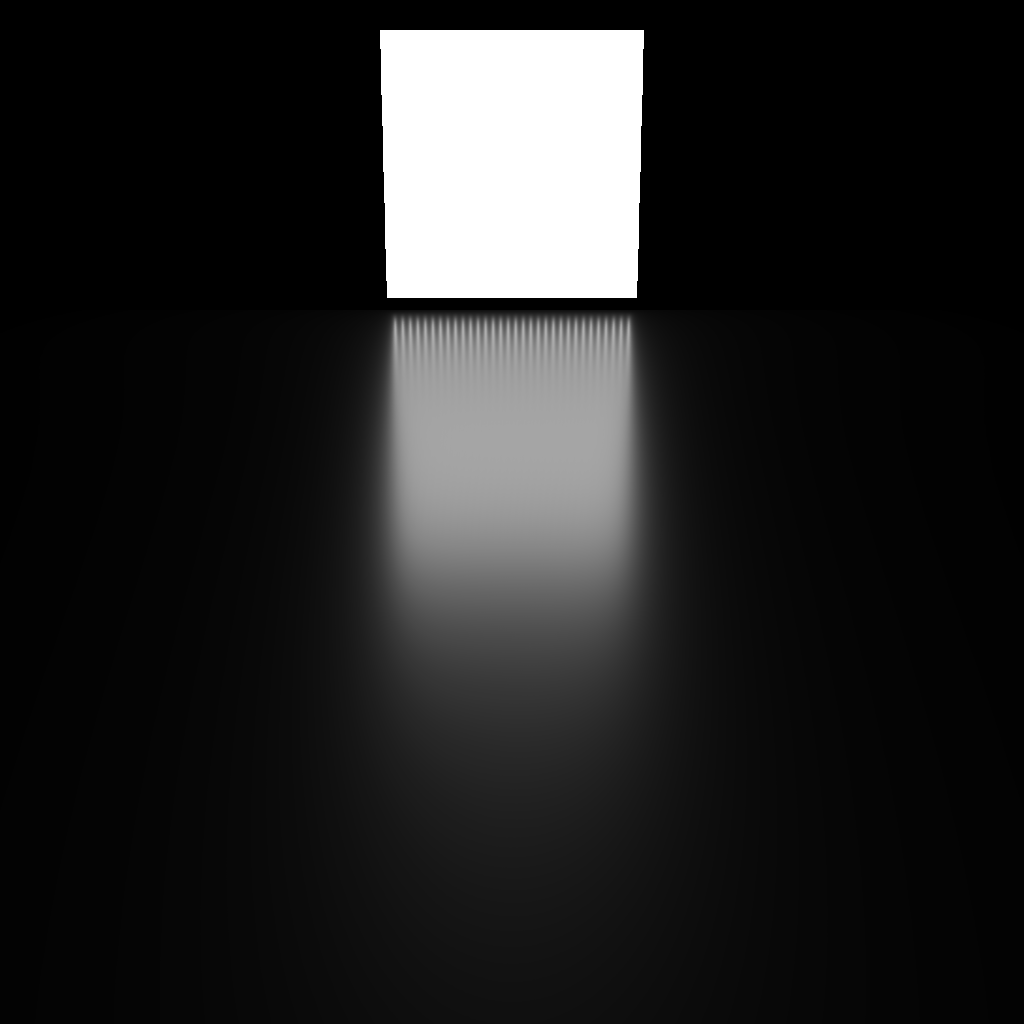
\includegraphics[width=\textwidth]{results/misc/point32x32-low-rough}
        \caption{32x32}
    \end{subfigure}
    \caption{Klastry świateł punktowych przy niskiej chropowatości. Opracowanie własne.}
    \label{fig:results:pointManyLowAlpha}
\end{figure}

\begin{table}
    \centering
    \begin{tabular}{|c|c|c|}
        \hline
        Metoda & Czas generacji & Maksymalny FPS \\ \hline
        Klaster świateł punktowych (4x4) & 16ms & 62 \\ \hline
        Klaster świateł punktowych (6x6) & 16ms & 62 \\ \hline
        Klaster świateł punktowych (8x8) & 16ms & 62 \\ \hline
        Klaster świateł punktowych (10x10) & 16ms & 62 \\ \hline
        Klaster świateł punktowych (12x12) & 17ms & 58 \\ \hline
        Klaster świateł punktowych (14x14) & 24ms & 41 \\ \hline
        Klaster świateł puntkowych (16x16) & 30ms & 33 \\ \hline
        Klaster świateł puntkowych (20x20) & 47ms & 21 \\ \hline
        Klaster świateł puntkowych (32x32) & 120ms & 8 \\ \hline
        Liniowo transformowane kosinusy & 16ms & 62 \\ \hline
        Monte-Carlo (12800 próbek)& 16442ms & 0.05 \\
        \hline
    \end{tabular}
    \caption{Czas potrzebny na wygenerowanie pojedynczej ramki o wymiarach 1024 na 1024 pikseli. Teoretyczny maksymalny FPS jest wynikiem $\left \lfloor \frac{1\text{s}}{\text{czas generowania ramki}}\right \rfloor$. Opracowanie własne.}
    \label{tab:performance}
\end{table}

\begin{table}[h]
    \centering
    \begin{tabular}{C{0.5cm}C{3cm}C{3cm}C{3cm}}
        $\alpha$ & Monte-Carlo & Światła punktowe (8x8) & LTC \\
        $0.05$ 
            & \includegraphics[width=3cm]{results/metal/{gt-flux-10-roughness-0.05}.png}
            & \includegraphics[width=3cm]{results/metal/{point8x8-flux-10-roughness-0.05}.png}
            & \includegraphics[width=3cm]{results/metal/{ltc-flux-10-roughness-0.05}.png} 
            \\
        $0.2$ 
            & \includegraphics[width=3cm]{results/metal/{gt-flux-10-roughness-0.2}.png}
            & \includegraphics[width=3cm]{results/metal/{point8x8-flux-10-roughness-0.2}.png}
            & \includegraphics[width=3cm]{results/metal/{ltc-flux-10-roughness-0.2}.png} 
            \\
        $0.4$ 
            & \includegraphics[width=3cm]{results/metal/{gt-flux-10-roughness-0.4}.png}
            & \includegraphics[width=3cm]{results/metal/{point8x8-flux-10-roughness-0.4}.png}
            & \includegraphics[width=3cm]{results/metal/{ltc-flux-10-roughness-0.4}.png} 
            \\
        $0.6$
            & \includegraphics[width=3cm]{results/metal/{gt-flux-10-roughness-0.6}.png}
            & \includegraphics[width=3cm]{results/metal/{point8x8-flux-10-roughness-0.6}.png}
            & \includegraphics[width=3cm]{results/metal/{ltc-flux-10-roughness-0.6}.png}
            \\
        $0.8$ 
            & \includegraphics[width=3cm]{results/metal/{gt-flux-10-roughness-0.8}.png}
            & \includegraphics[width=3cm]{results/metal/{point8x8-flux-10-roughness-0.8}.png}
            & \includegraphics[width=3cm]{results/metal/{ltc-flux-10-roughness-0.8}.png}
            \\
        $1.0$ 
            & \includegraphics[width=3cm]{results/metal/{gt-flux-10-roughness-1}.png}
            & \includegraphics[width=3cm]{results/metal/{point8x8-flux-10-roughness-1}.png}
            & \includegraphics[width=3cm]{results/metal/{ltc-flux-10-roughness-1}.png}
    \end{tabular}
    \caption{Jednolita metalowa powierzchnia o różnym współczynniku chropowatości $\alpha$. Opracowanie własne.}
    \label{tab:results:metal}
\end{table}

\begin{table}[h]
    \centering
    \begin{tabular}{C{0.5cm}C{3cm}C{3cm}C{3cm}}
    $\alpha$ & Monte-Carlo & Światła punktowe (8x8) & LTC \\
    $0.05$ 
        & \includegraphics[width=3cm]{results/isolator/{gt-flux-10-roughness-0.05}.png}
        & \includegraphics[width=3cm]{results/isolator/{point8x8-flux-10-roughness-0.05}.png}
        & \includegraphics[width=3cm]{results/isolator/{ltc-flux-10-roughness-0.05}.png} 
        \\
    $0.2$ 
        & \includegraphics[width=3cm]{results/isolator/{gt-flux-10-roughness-0.2}.png}
        & \includegraphics[width=3cm]{results/isolator/{point8x8-flux-10-roughness-0.2}.png}
        & \includegraphics[width=3cm]{results/isolator/{ltc-flux-10-roughness-0.2}.png} 
        \\
    $0.4$ 
        & \includegraphics[width=3cm]{results/isolator/{gt-flux-10-roughness-0.4}.png}
        & \includegraphics[width=3cm]{results/isolator/{point8x8-flux-10-roughness-0.4}.png}
        & \includegraphics[width=3cm]{results/isolator/{ltc-flux-10-roughness-0.4}.png} 
        \\
    $0.6$
        & \includegraphics[width=3cm]{results/isolator/{gt-flux-10-roughness-0.6}.png}
        & \includegraphics[width=3cm]{results/isolator/{point8x8-flux-10-roughness-0.6}.png}
        & \includegraphics[width=3cm]{results/isolator/{ltc-flux-10-roughness-0.6}.png}
        \\
    $0.8$ 
        & \includegraphics[width=3cm]{results/isolator/{gt-flux-10-roughness-0.8}.png}
        & \includegraphics[width=3cm]{results/isolator/{point8x8-flux-10-roughness-0.8}.png}
        & \includegraphics[width=3cm]{results/isolator/{ltc-flux-10-roughness-0.8}.png}
        \\
    $1.0$ 
        & \includegraphics[width=3cm]{results/isolator/{gt-flux-10-roughness-1}.png}
        & \includegraphics[width=3cm]{results/isolator/{point8x8-flux-10-roughness-1}.png}
        & \includegraphics[width=3cm]{results/isolator/{ltc-flux-10-roughness-1}.png}
    \end{tabular}
    \caption{Izolator o różnym współczynniku chropowatości $\alpha$. Opracowanie własne.}
    \label{tab:results:isolator}
\end{table}

\begin{table}[h]
    \centering
    \begin{tabular}{C{2cm}C{3cm}C{3cm}C{3cm}}
    Rodzaj & Monte-Carlo & Światła punktowe (8x8) & LTC \\
    Żelazo 
        & \includegraphics[width=3cm]{results/textured/{gt-scuffed-iron}.png}
        & \includegraphics[width=3cm]{results/textured/{point8x8-scuffed-iron}.png}
        & \includegraphics[width=3cm]{results/textured/{ltc-scuffed-iron}.png}
        \\
    Miedź 
        & \includegraphics[width=3cm]{results/textured/{gt-polished-copper}.png}
        & \includegraphics[width=3cm]{results/textured/{point8x8-polished-copper}.png}
        & \includegraphics[width=3cm]{results/textured/{ltc-polished-copper}.png}
        \\
    Polypropylen 
        & \includegraphics[width=3cm]{results/textured/{gt-polypropylene}.png}
        & \includegraphics[width=3cm]{results/textured/{point8x8-polypropylene}.png}
        & \includegraphics[width=3cm]{results/textured/{ltc-polypropylene}.png}
        \\
    Marmur
        & \includegraphics[width=3cm]{results/textured/{gt-marble-checkerboard}.png}
        & \includegraphics[width=3cm]{results/textured/{point8x8-marble-checkerboard}.png}
        & \includegraphics[width=3cm]{results/textured/{ltc-marble-checkerboard}.png}
        \\
    Kafelki
        & \includegraphics[width=3cm]{results/textured/{gt-vintage-tiles}.png}
        & \includegraphics[width=3cm]{results/textured/{point8x8-vintage-tiles}.png}
        & \includegraphics[width=3cm]{results/textured/{ltc-vintage-tiles}.png}
    \end{tabular}
    \caption{Różne materiały opisane teksturami. Wykorzystane tekstury pochodzą ze strony \url{http://freepbr.com} oraz \url{http://textures.com}. Opracowanie własne.}
    \label{tab:results:textured}
\end{table}

\begin{figure}[h]
    \centering
    \includegraphics[width=\linewidth]{results/misc/fit_matrix}
    \caption{Wizualne porównanie oryginalnej odpowiedzi BRDF (GGX) oraz wyznaczonego przybliżenia LTC. Od lewej do prawej zwiększa się kąt obserwacji, od góry do dołu rośnie chropowatość powierzchni. Pary wierszy obrazują wynik dla tego samego parametru chropowatości. Opracowanie własne.}
    \label{fig:results:fitMatrix}
\end{figure}

\end{document}
